\documentclass{sprawozdanie-agh}

\usepackage[utf8]{inputenc}
\usepackage{listings}
\usepackage{pdfpages}
\usepackage{float}
\usepackage{anyfontsize}
\usepackage{graphicx}
 
\makeatletter 

\begin{document}   

	\przedmiot{Wprowadzenie do wzorców projektowych}
	\tytul{,,Tablica ogłoszeń''}
	\podtytul{Implementacja mechanizmu server-push z wykorzystaniem techniki streaming w technologii
		ReactJS oraz NodeJS.}
	\kierunek{Informatyka, III rok, 2018/2019}
	\autor{Agnieszka Zadworny, Maciej Bielech, Tomasz Pęcak, Piotr Morawiecki}
	\data{Kraków, 13 lutego 2019}

	\stronatytulowa{}
	\section{Informacje ogólne}
	
	\subsection{Cel projektu}
	Celem projektu jest zaimplementowanie metody Server Push w technice streaming przy użyciu technologii NodeJS i ReactJS.
	
	\subsection{Opis aplikacji}
	Utworzona została aplikacja webowa o nazwie ,,Tablica ogłoszeń'', która umożliwia publikowanie ogłoszeń o wybranej tematyce. Klient otwierając stronę aplikacji otrzymuje listę ogłoszeń sortowaną od najnowszego, jeśli w czasie przebywania na witrynie pojawi się nowe ogłoszenie, serwer wyśle jego treść dzięki wykorzystaniu techniki Server Push, która została zaimplementowana przy użyciu websocketów. 
	
	\subsection{Server Push}
	Push technology, czyli server push, to styl komunikacji internetowej, w którym żądanie danej transakcji jest inicjowane przez serwer. W przeciwieństwie do pull/get, gdzie żądanie przekazania informacji jest inicjowane przez odbiorcę lub klienta.
	
	Usługi Push są często oparte na preferencjach informacyjnych wyrażanych z wyprzedzeniem. Nazywa się to modelem publikacji/subskrybcji. Klient "subskrybuje" różne "kanały" informacyjne dostarczane przez serwer; gdy na jednym z tych kanałów dostępne są nowe treści, serwer "pushuje" te informacje do klienta.
	
	\subsection{Websocket}
	Protokół WebSocket umożliwia interakcję między klientem internetowym (np. przeglądarką), a serwerem WWW przy dokonywaniu mniejszej ilości zapytań, ułatwiając przesyłanie danych w czasie rzeczywistym z i na serwer. Jest to możliwe dzięki zapewnieniu znormalizowanego sposobu, w jaki serwer może wysyłać treści do klienta bez uprzedniego żądania z jego strony i pozwalającego na przekazywanie wiadomości w obu kierunkach przy zachowaniu otwartego połączenia. W ten sposób może mieć miejsce dwukierunkowe połączenie pomiędzy klientem i serwerem. 
	
	
	\section{Jak korzystać z biblioteki socket-lib}
	
	\section{Jak korzystać z biblioteki socket-lib-client}
	
	\section{Wykorzystane wzorce projektowe}
	\subsection{Fasada}
	
	Korzystamy z niej aby dostarczyć klientowi uproszczony interfejs biblioteki socket-io
	
	\begin{figure}[H] 
		\centering
		\begin{tabular}{c}
			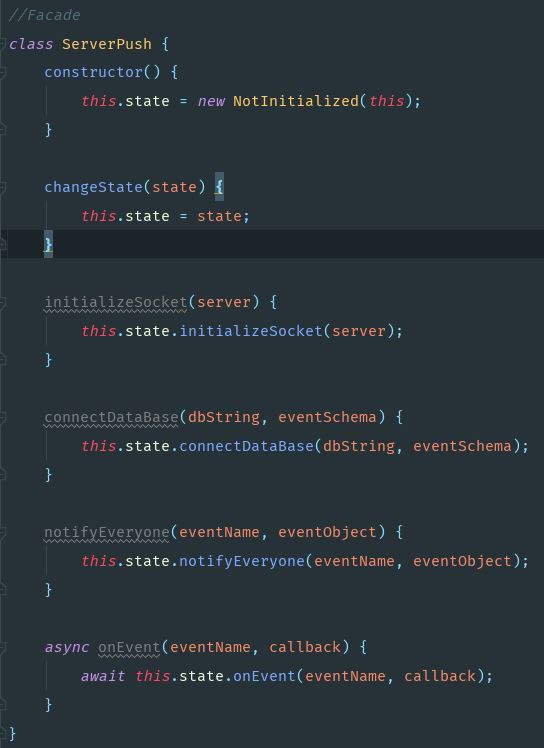
\includegraphics[width=.75\textwidth]{Fasada}
		\end{tabular} 
		\caption{Implementacja fasady}
	\end{figure}
	
	\begin{figure}[H] 
		\centering
		\begin{tabular}{c}
			\includegraphics[width=.75\textwidth]{Fasadaclass}
		\end{tabular} 
		\caption{Diagram klas fasady}
	\end{figure}
	
	\subsection{Query Builder}
	
	Obiekt reprezentuje zapytanie kierowane do bazy
	danych. Generuje zapytanie SQL, bazując na klasach i polach
	klas.Uzyskaliśmy dzięki niemu niezależność aplikacji od schematu
	bazy danych. Dodatkowo pozwala on na korzystanie z różnych motorów baz danych.
	
	\begin{figure}[H] 
		\centering
		\begin{tabular}{c}
			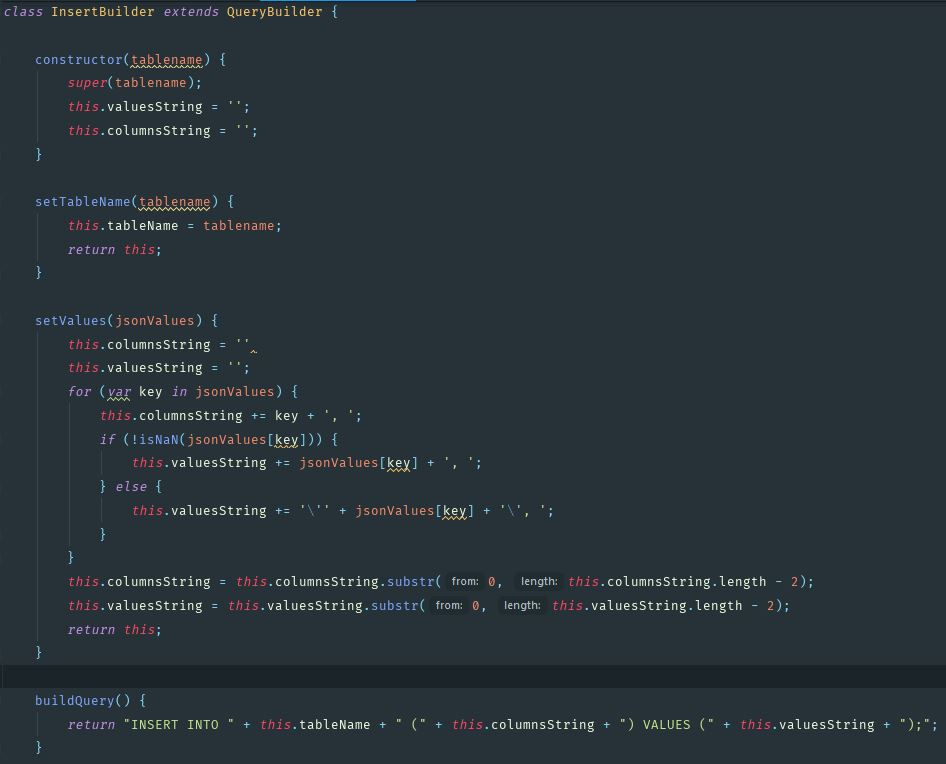
\includegraphics[width=.99\textwidth]{insertbuilder}
		\end{tabular} 
		\caption{Implementacja Query Builder'a}
	\end{figure}

	\begin{figure}[H] 
		\centering
		\begin{tabular}{c}
			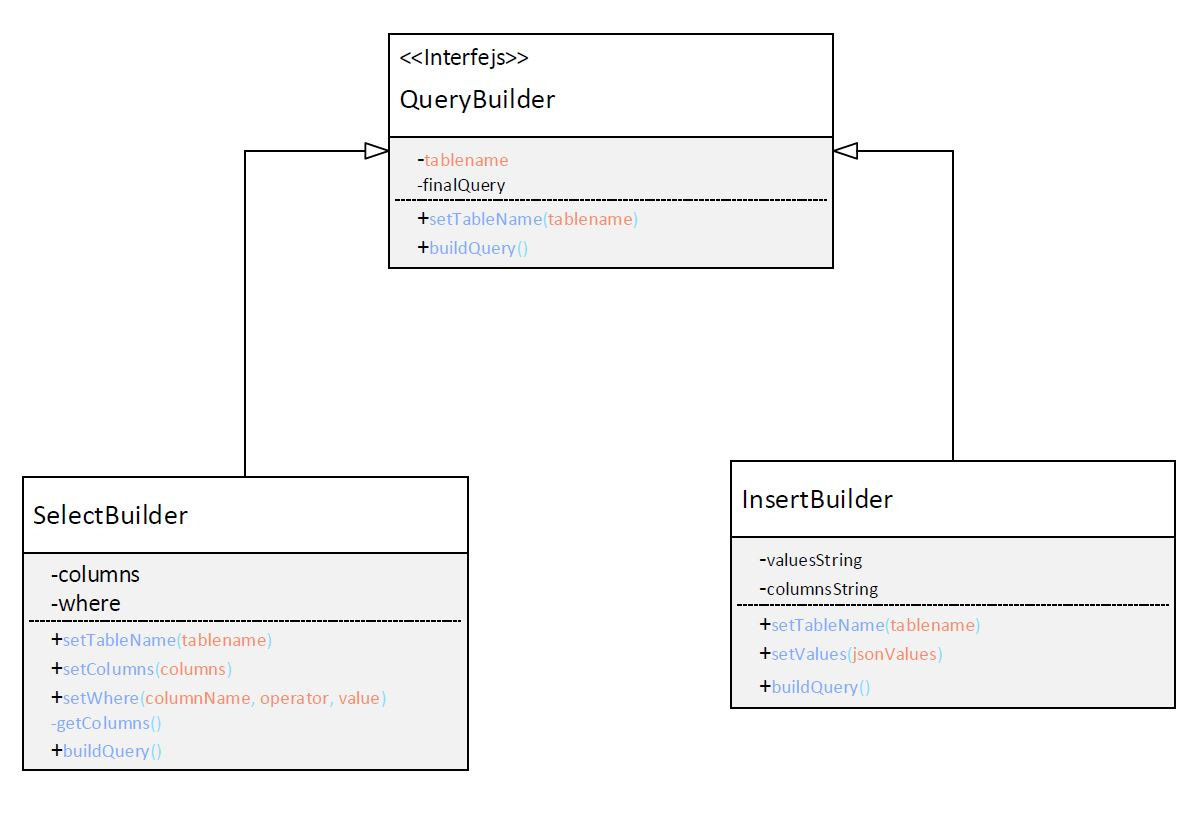
\includegraphics[width=.99\textwidth]{querybuilder}
		\end{tabular} 
		\caption{Diagram klas Query Builder'a}
	\end{figure}
	
	\subsection{Fabryka Abstrakcyjna}
	
	Wzorzec wymusza zależności pomiędzy	klasami konkretnymi – zależności obiektów w rodzinie co w naszym przypadku jest pożądane, bo otrzymamyy obiekty ze sobą kompatybilne.
	
	\begin{figure}[H] 
		\centering
		\begin{tabular}{c}
			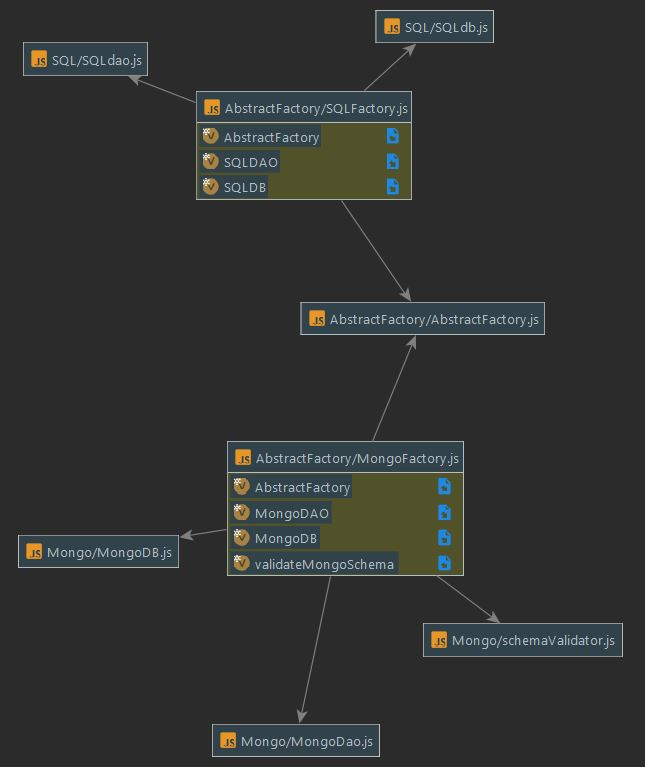
\includegraphics[width=.95\textwidth]{abstractfactory}
		\end{tabular} 
		\caption{Diagram klas dla fabryki abstrakcyjnej}
	\end{figure}
	
	\subsection{Singleton}
	
	\begin{figure}[H] 
		\centering
		\begin{tabular}{c}
			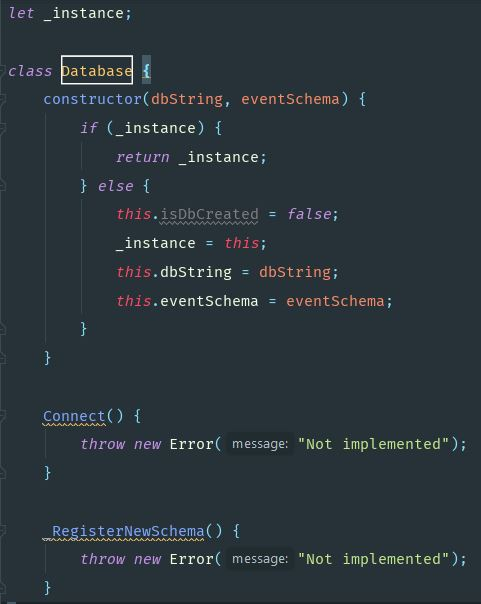
\includegraphics[width=.75\textwidth]{singleton}
		\end{tabular} 
		\caption{Implementacja fabryki abstrakcyjnej jako singletona}
	\end{figure}
	
	\subsection{Maszyna Stanowa}
	
	\begin{figure}[H] 
		\centering
		\begin{tabular}{c}
			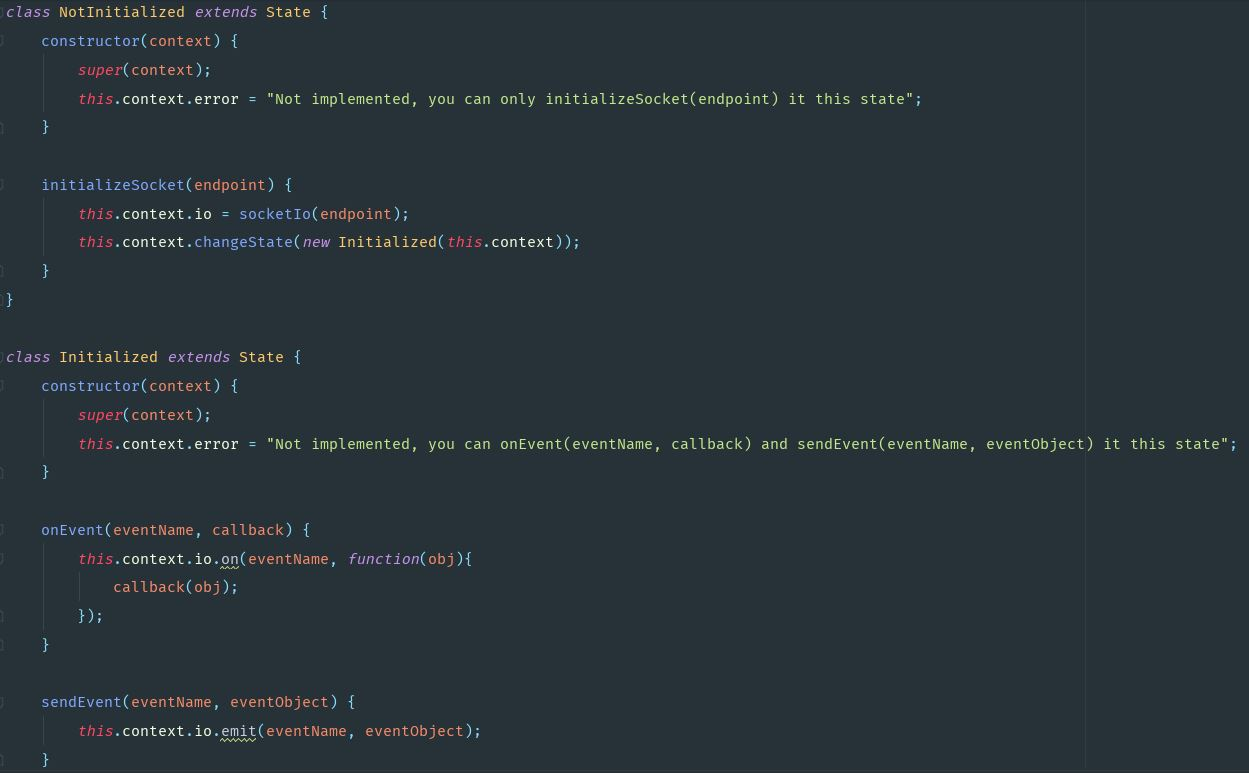
\includegraphics[width=.99\textwidth]{statemachine}
		\end{tabular} 
		\caption{Implementacja maszyny stanowej}
	\end{figure}

	\begin{figure}[H] 
		\centering
		\begin{tabular}{c}
			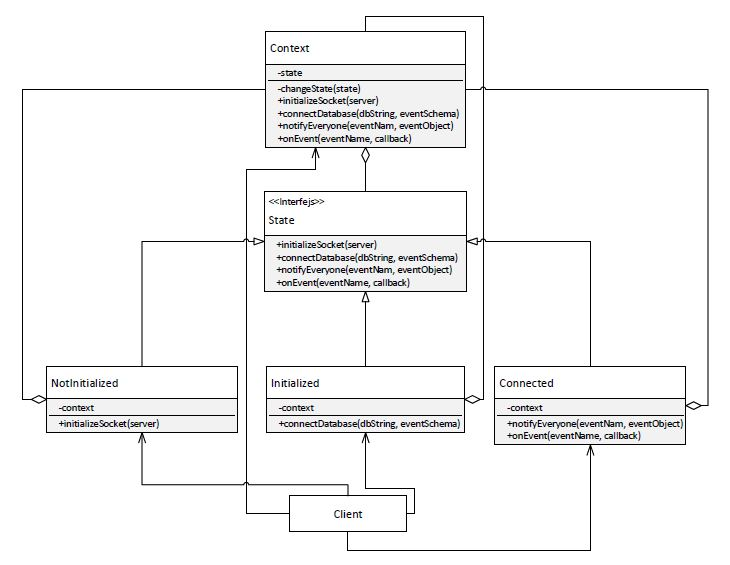
\includegraphics[width=.99\textwidth]{statemachineclass}
		\end{tabular} 
		\caption{Diagram klas maszyny stanowej}
	\end{figure}

	\subsection{Dao Factory}
	
	\begin{figure}[H] 
		\centering
		\begin{tabular}{c}
			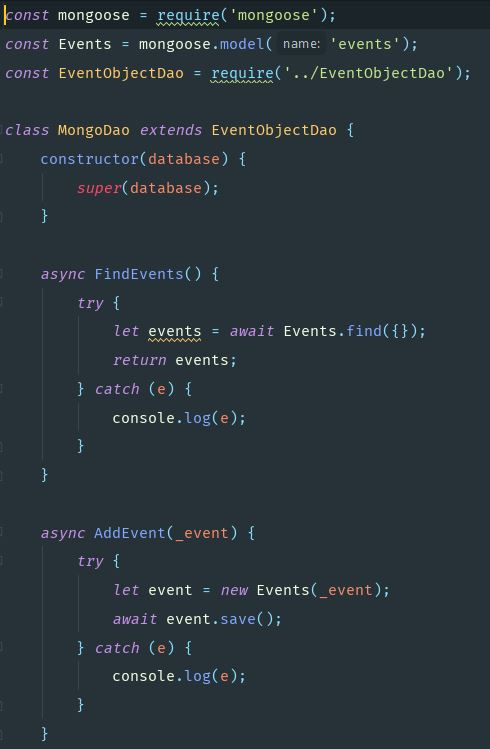
\includegraphics[width=.75\textwidth]{mongodao}
		\end{tabular} 
		\caption{Implementacja DAO Factory}
	\end{figure}


\end{document}